\chapter{Introduction}
\label{chapter:introduction}

Twenty years after its birth, the Web has become one of the defining
technological innovations that knows no geographical, political, or
ideological boundaries. The world wide platform built on top of the
physical Internet is deeply integrated into our daily lives. This
powerful tool that was built on egalitarian principles is now taken
for granted, just like old innovations such as
electricity. \cite{berners2010long}

In parallel with the rapid growth of the Web, mobile phones have
evolved from briefcase-sized ``portable'' telephony devices into
modern pocket-sized computers. The mobile revolution has already
changed the world as we see it, and more people have access to the Web
from a mobile device than from an Internet-connected desktop
computer. \cite{fling2009mobile}

The Web is not constrained into (desktop and laptop) computers and
mobile phones, though. Tablets, TVs, ebook readers, watches, and even
household appliances are connecting to the Internet and have web
browsers. For the first time in history, we have a truly ubiquitous
digital medium. \cite{fling2009mobile}

Universal accessibility and openness are the keys to being the
ubiquitous information platform of the digital age
\cite{berners2010long}. Now the Web is closer in accomplishing its
original principles in equality and universality; anyone can access
this vast source of open information from anywhere, with any
device. All you need is a web browser that supports the open standards
of the Web.

\begin{quotation}
  \noindent \textit{The goal of the Web is to serve humanity.}
  \begin{flushright}
    -- Tim Berners-Lee \cite{berners2010long}
  \end{flushright}
\end{quotation}

Being the universal digital medium, mobile devices has some unique
characteristics that other mass media lack. Mobile is personal,
always-on, always-carried medium with a built-in payment
channel. Mobile is in your pocket at the moment you have your creative
impulse. \cite{fling2009mobile}

These characteristics have made mobile device applications a
multibillion-dollar business. Five years after Apple published its
game-changing iPhone and the App Store, touch screen mobile phones and
tablets from different device manufacturers have spread all over the
world. \cite{cortimiglia2011mobile, charland2011mobile,
  fling2009mobile}

However, this proliferation of mobile devices and platforms has raised
a serious issue for application developers: fragmentation. Not only
are there multiple target platforms, but even within the platforms
there are different versions with different feature sets, not to
mention different devices with varying
capabilities. \cite{charland2011mobile}

\begin{table}
  \begin{tabular}{ l | l }
    \textbf{Mobile OS Type} & \textbf{Skill Set Required} \\
    \hline
    Apple iOS & C, Objective C \\
    Google Android & Java (Harmony flavored, Dalvik VM) \\
    RIM BlackBerry & Java (J2ME flavored) \\
    Symbian & C, C++, Python, HTML/CSS/JS \\
    Windows Mobile & .NET \\
    Windows 7 Phone & .NET \\
    HP Palm webOS & HTML/CSS/JS \\
    MeeGo & C, C++, HTML/CSS/JS \\
    Samsung bada & C++
  \end{tabular}
  \label{table:native-skills}
  \caption{Required developer skill sets for different mobile
    platforms according to \cite{charland2011mobile}}
\end{table}

Table~\ref{table:native-skills} (\fixme{check table ref number}) shows
the required developer skill sets for different platforms. As we see,
each platform has its own programming language and \abbr{SDK}. A lot
of knowledge and resources are needed to provide cross-platform
applications for these platforms. Making several independent
applications with the native tools is also very expensive, and adding
features or just maintaining all these different applications becomes
costly. \cite{charland2011mobile}

Some developers are forced to make compromises due to resourcing or
budgeting, and build their applications only for one platform. This
might be fine for independent developers, but a lot of potential
customers or users are left out of these walled gardens. Big
corporations or public organizations cannot afford leaving out large
shares of the mobile market. \cite{berners2010long}

\fixme{add platform market share figure}

Being cross-platform is essential in today's mobile market. And if the
required skills and resources for the native tools are not present,
other options have to be considered. All mobile devices have a web
browser, and the Web is becoming the universal application
platform. \cite{taivalsaari2011web, mikkonen2011apps}

In the 20 years of its lifetime, the Web has evolved from a simple
system for sharing documents into a massively popular, world wide
application and information distribution environment
\cite{taivalsaari2011web}. During the so-called Web 2.0 revolution,
the Web grew into a platform for interactive applications with the
help of technologies like \abbr{Ajax} \cite{garrett2005ajax}.

The Web is not without its problems, however. The viral spreading of
mobile phones has raised the need for a feature-rich technology stack
for building scalable applications that can handle the whole spectrum
of devices, screen sizes, and form factors that are used to access the
Internet. This is the need that \abbr{HTML5} with all the related
tools and \abbr{APIs} have promised to solve.

Performance is the foundation of a great user experience
\cite{charland2011mobile}. By performance we mean the speed of
downloading, initializing and using an application as perceived by the
user as well as the responsiveness and smoothness of the user
interface influencing the overall user experience.

Native tools have been carefully optimized to provide the best
possible performance and responsiveness, and web applications are
often unfavorably compared to them. In the end, however, the received
savings in development time, deployment, cost-efficiency, and
cross-platform support can often outweigh the possible
compromises. \cite{charland2011mobile, fling2009mobile}

In this work we look at the performance of \abbr{HTML5} as a
cross-platform application platform for different device
form-factors. To study the performance, we built a real world HTML5
application and a JavaScript library and fine-tuned the performance to
get the best possible user experience. We then asses these
optimizations and the compromises that had to be made.

\fixme{Add more about background and objectives of this work}

\section{Research Question}

Assuming that we know the reasons and motivation for cross-platform
HTML5 and the importance of application performance and
responsiveness:

\begin{itemize}
\item How should we build cross-platform HTML5 applications?

  \begin{itemize}
  \item How can we optimize the user interface performance?
  \item How can we handle the flaky and slow mobile networks?
  \item How can we handle different screen sizes and device types?
  \end{itemize}
\end{itemize}

\noindent In other words, we know the Why, but what about the How?

\chapter{Specifications}
\label{chapter:specifications}

\section{HTML5}
\label{section:html5}

HTML5 is a cross-platform and device form-factor agnostic markup
language for defining structured documents. It is a backward
compatible revision of older HTML standards bringing lots of new
functionality, removing unneeded features, and officially documenting
some ``de facto'' standards already supported by some or several web
browsers. \cite{pilgrim2010html5}

In the early 2000s, \abbr{W3C} was developing \abbr{XHTML} and
\abbr{XForms} standards to be the future of the Web. Many parts of
these standards were backward incompatible and required very strict
and error-free authoring. Being frustrated with this vision that was
seen as impractical for the real world, a group of web browser vendors
and other interested parties had a competing vision of the future of
the Web: evolving HTML4 to include additional features maintaining
backward compatibility. W3C members did not agree with this vision,
and as a result, the WHAT Working Group was born. \abbr{WHATWG} is a
``loose, unofficial, and open collaboration of Web browser
manufacturers and interested
parties''\footnote{\url{http://www.whatwg.org/news/start}}. \cite{pilgrim2010html5}

According to a
study\footnote{\url{http://dev.opera.com/articles/view/mama-key-findings/}}
made by Opera in 2008, more than 95\% of web sites do not pass markup
validation. Therefore, to maintain backward compatibility and
practicality, it is crucial to have a well defined error handling
mechanism.

Having the browser vendor and web development community support behind
them, after several years the WHATWG work was finally accepted by W3C
and a joint effort was started to standardize HTML5. There are still
differences in the W3C and WHATWG specifications in what features they
include in the main standard and what are separated in other
specifications or leaved out, but the main goal is to develop the
standards together with browser vendors to get usage feedback while
the specifications are being made. This results in many features being
available in modern web browsers while the HTML5 and related standards
are not yet finished. As a drawback, however, the implementations
might change between browser versions, and developers must take extra
effort in detecting the supported features. \cite{pilgrim2010html5}

In this work, we look at HTML5 beyond the main specifications, and
take into account also related standards that affect modern web
application development. Also, the differences between the W3C and the
WHATWG specifications are not separated since they are not
clear-cut. This is the practical view that, in our opinion, the web
development community has on HTML5.

\subsection{Semantic Markup}

Google did a study\footnote{\url{http://code.google.com/webstats/}} in
2005 of a sample of over a billion HTML documents about the popular
class names, elements, attributes and related metadata. This analysis
had a large impact on which elements and attributes were considered in
the upcoming HTML5 standard.

HTML5 defines several new elements and attributes. The objective is to
make the markup more semantic for developers and for content
processors such as search engines and screen readers.

The specification aims for a more semantic structure of HTML by
dropping many presentational features. The rationale behind this is
explained with the following reasons \cite{HTML5draft}:

\begin{itemize}
\item Media-independent markup works for more users and yields better
  accessibility
\item Having style-independent markup separates document structure
  from its layout and makes maintenance easier
\item Separating styling results in smaller document sizes.
\end{itemize}

\noindent Each element in HTML5 is in zero or more content categories
that group elements with similar characteristics \cite{HTML5draft}:

\begin{itemize}
\item \textbf{Metadata content:} Content that sets the behavior of the
  document, sets its relationships to other documents, or conveys
  other information of the document.

  \textit{Examples:} \texttt{link}, \texttt{meta}, \texttt{script},
  \texttt{title}

\item \textbf{Flow content:} Most content that is used in the body of
  a document.

  \textit{Examples:} \texttt{a}, \texttt{article}, \texttt{audio},
  \texttt{div}, \texttt{header}, \texttt{form}, \texttt{nav},
  \texttt{p}

\item \textbf{Sectioning content:} Content that defines the scope of
  headings and footers.

  \textit{Examples:} \texttt{article}, \texttt{aside}, \texttt{nav},
  \texttt{section}

\item \textbf{Heading content:} Content that defines a header of a
  section.

  \textit{Examples:} \texttt{h1}, \texttt{h2}, \texttt{hgroup}

\item \textbf{Phrasing content:} Content that holds or marks up the
  text of the document.

  \textit{Examples:} \texttt{abbr}, \texttt{audio}, \texttt{canvas},
  \texttt{img}, \texttt{em}

\item \textbf{Embedded content:} Content that imports another resource
  or inserts content from another vocabulary into the document.

  \textit{Examples:} \texttt{audio}, \texttt{embed}, \texttt{iframe},
  \texttt{img}

\item \textbf{Interactive content:} Content that is intended for user
  interaction.

  \textit{Examples:} \texttt{a}, \texttt{button}, \texttt{menu},
  \texttt{select}

\end{itemize}

\subsection{Extensibility}

HTML5 defines the main constructs of a semantic and accessible
document. However, some specific use cases require a more precise and
context-dependent and fine-grained semantics. Also, web browsers might
introduce new features that must conform to the standards. This is why
HTML5 is made extensible for adding more semantics or additional
features on top of the existing standard.

There are several ways to extend HTML5. The simplest approaches
include using the defined general attributes with certain
vocabularies. For example,
microformats\footnote{\url{http://microformats.org/}} and
Schema.org\footnote{\url{http://schema.org/}} define common elements
and class names with certain semantics for defining document metadata.

HTML5 also defines explicit mechanisms for extending the markup
structure. Using \texttt{data-*=""} and \texttt{rel} attributes,
\texttt{meta} tags, or a generic microdata mechanism, the semantics of
the content can be enhanced for automatic reasoning and machine
readability. \cite{HTML5draft}

\subsection{Media}

Multimedia support is crucial for modern applications. HTML5 defines
elements and APIs for audio, video, subtitles, and embedded content.

Previously to use these rich content types, developers have had to
rely on third-party plugins and browser extensions. Not having to rely
on plugins and extensions has been one of the main goals of the HTML5
standard for improving the openness and accessibility of web content.

\subsection{Canvas 2D Context}

HTML5 defines the \texttt{canvas} element. It is a
resolution-dependent bitmap canvas for dynamically rendering
graphics. It can be used, for example, for graphs, games, or other
visuals. \cite{HTML5draft}

The Canvas 2D Context specification draft \cite{canvas2Ddraft} defines
a JavaScript API for programmatically drawing on the 2D canvas
surface. The API defines functions for drawing shapes, paths, text,
gradients, and images on the canvas and other functions for handling
the bitmap data.

\subsection{Form Enhancements}

Forms are an essential construction in interactive HTML
documents. However, due to their relative simplicity in terms of
expressiveness and the lack of proper accessibility features,
developers have been forced to build lots of JavaScript solutions to
enhance and fix some of these problems.

HTML5 brings several enhancements to forms. New input types for
numbers, dates, email addresses, etc. obsolete the need of scripted
widgets by using native platform controls. New form attributes like
\texttt{placeholder} and \texttt{autofocus} bring easy-to-use
accessibility and usability improvements and also diminish the need
for scripting. \cite{HTML5draft}

These additions and enhancements work especially well in mobile
context where user input is slow and cumbersome. For example, by
having a numeric input field lets the mobile platform open the numeric
keyboard by default, which greatly improves the usability of
forms. Automatic form validation in the client side also reduces the
need for unneeded page refreshes since the browser can show error
messages in invalid fields without any JavaScript validation.

\subsection{Session History Manipulation}

HTML was originally designed to be based on documents and hyperlinks
between these distinct documents with each of them having a unique
\abbr{URL}. This hyperlinked structure, however, does not suit well
for web applications with dynamic content and interactively changing
user interface.

Two of the basic functionalities that users are accustomed to are
bookmarking and going back in the session history. Traditionally these
have been compromised in dynamic \abbr{Ajax} applications or handled
with a lot of extra work.

HTML5 addresses these issues by allowing the developers dynamically
manipulate the session history. The history stack can be changed and
used for navigation and even the browser address bar can be changed
without extra page refreshes. \cite{HTML5draft}

\subsection{Offline Web Applications}

By design, web sites have always needed a working network
connection. Applications, however, should be able to work offline or
in unreliable and flaky networks. Especially mobile networks are
unreliable \citationneeded, which has raised the need for offline
support in HTML5.

There are several ways to enable offline support in HTML5
applications. We present these approaches in the following sections.

\subsubsection{Application Cache}
\label{section:appcache}

\abbr{AppCache} is a relatively simple way to indicate all resources
needed for offline functionality. A manifest file is defined in the
HTML document, and within the file there are sections for resources
that should always or never be cached as well as fallback \abbr{URLs}
for resources that are not cached but with which the fetching
fails. In addition to the simple manifest file listing offline
resources, JavaScript events are defined for cache
changes. \cite{HTML5draft} \\

\noindent \textbf{Example manifest file:}
\begin{verbatim}
CACHE MANIFEST

# Example manifest version 1.

# The resources in this section are cached for offline use.
CACHE:
js/scripts.js
css/styles.css
img/sprite.png
http://example.org/external-image.jpg

# The resources in this section require the user to be online.
NETWORK:
/login

# This section defines resources and their fallback
# URLs if they are inaccessible.
FALLBACK:
/ /offline.html
\end{verbatim}

\subsubsection{Data Storage}
\label{section:datastorage}

Storing data in the client side has traditionally been constrained
into using cookies, but HTML5 specifies new options for data
persistence.

Two different key/value storages are defined: \texttt{localStorage}
and \texttt{sessionStorage}. The \abbr{API} is same with both of
these, but with \texttt{sessionStorage}, the data is persisted only
for the current browser session. These interfaces are very simple and
easy to use, but are constrained into storing only textual
data. \cite{webstoragedraft}

Two more expressive storage \abbr{APIs} have been specified: client
side \abbr{SQL} database \cite{webstoragedraft} and the Indexed
Database \cite{indexedDBdraft}. The client side SQL database defines
an asynchronous and transactional JavaScript API for a SQL
database. Although being very expressive, due to the relative
complexity compared to simple and scalable key/value storage options,
it is yet to be seen if the client side SQL storage will be accepted
by the browser vendors and developers.

Indexed Database provides synchronous and asynchronous APIs for
storing and querying large amounts of structured data. The
transactional API can be used for more complex persistency needs than
with the simple key/value storages, and it provides a native
JavaScript API that does not involve the relative complexities of SQL.

\subsubsection{Detecting Network State}

Knowing whether the user is online or offline can affect the user
interface or the response to user interactions. HTML5 defines
functionality to detect the current network status and events that are
fired when the status changes. \cite{HTML5draft}

Although providing important information, these network status
indicators are inherently unreliable \cite{HTML5draft}. Due to the
distributed ad-hoc architecture of the network and possible local or
external proxies or middleware, the application can never be sure if
the network is connected or not. The only option is just to attempt to
make requests and wait for the response or possible failure.

Therefore, applications should be designed to expect the network to
work, but to degrade gracefully when the connection is lost or seems
to be unreliable.

\subsection{Drag and Drop}
\label{section:dragdrop}

Drag and Drop is a common interaction technique where elements can be
moved within the user interface from one place to another. Older
browsers have had proprietary solutions for this interaction pattern,
but HTML5 standardizes the API.

The specification defines the element attributes and \abbr{DOM} events
for easily enabling and controlling draggable elements and drop
targets. Custom cross-browser JavaScript solutions have enabled this
interaction before, but little JavaScript code is needed with the new
API. The browser handles the interaction and the dynamic rendering,
reducing the interface lagging and the need for extra processing.

\subsection{SVG and MathML}

While not part of the HTML5 standard, the specification allows for
embedding \abbr{SVG} \cite{SVGTiny12} and \abbr{MathML} \cite{MathML}
markup within HTML.

SVG is a markup language for describing two-dimensional vector
graphics in \abbr{XML}. The markup can be accessed with the \abbr{DOM}
API for creating dynamic and interactive functionality. Within an
HTML5 document, SVG markup can be embedded within the \texttt{svg}
element.

MathML is an \abbr{XML} markup language for describing the structure
and content of mathematical notation. It can be embedded within an
HTML5 document with the \texttt{math} element.

Both of these languages reduce the need of custom images, making the
content more accessible, dynamic, and enabling dynamic interaction
with it. Also, vector graphics can be scaled to fit the available
space no matter the screen size, which improves the cross-platform
usefulness for different device form factors.

\section{Other Related Specifications}

There are lots of specifications related to HTML5 that are considered
to be part of the practical view of all the new Web APIs that are
often referred to as 'HTML5'. Some of these originate from the work of
the \abbr{WHATWG} and some from the work of \abbr{W3C}, some have been
part of HTML5 at some point but have been taken out of it into their
own separate specifications, and some are just new specifications for
the Web that relate to what we can do with HTML, CSS, and JavaScript
in modern web applications. In the following sections, we introduce
the specifications that are of interest within the topic of this work.

\subsection{Cascading Style Sheets}
\label{section:css}

\abbr{CSS} Level 3 specifications introduce lots of new functionality
for web application styling. Well separated layout layer keeps the
document structure clean, and rich styling and effects capabilities
reduce the need for scripting and provide graceful fallback
functionality for older user agents. By letting the browser handle,
for example, rich user interface animation effects allows developers
to easily optimize the responsiveness and performance of their
applications since the browser can use the most efficient techniques
of the platform to handle these effects. Below we list the main
components and specifications of the \abbr{W3C} CSS working
group\footnote{\url{http://www.w3.org/Style/CSS/members.en.php3}}.

\begin{itemize}

\item \textbf{Selectors}

  \abbr{CSS} selectors are patterns that are used to match elements in
  a \abbr{DOM} tree. The patterns can then be used to apply style
  rules to the matched elements. Selectors can also be used in
  JavaScript to select elements for scripting.

  \abbr{CSS3} defines a set of new selectors \cite{CSS3Selectors} for
  powerful matching of elements in complex DOM trees. These selectors
  are useful for rich interactive web applications and reduce the need
  for scripting for element matching. Efficient selectors are also
  crucial for performance optimization.

\item \textbf{Transforms}

  2D and 3D transforms \cite{CSStransforms} allow elements to be
  transformed in two-dimensional or three-dimensional space. Elements
  can be translated, rotated, and scaled in their coordinate
  space. The specification defines lots of 2D and 3D transformation
  functions, which can be used in the transforms.

  Transforms can provide subtle but important user interface effects,
  or they can be used for advanced interactive graphics. Combined
  with, for example, timed animations or transitions, rich user
  interfaces can be built with declarative CSS rules.

\item \textbf{Transitions}

  CSS transitions \cite{CSStransitions} allow element styles to change
  smoothly over a specified duration, and they can be used for simple
  animations. Normally when the value of a CSS property changes, the
  result is seen instantly, but with transitions, the changes can be
  timed and configured for presentational effects.

\item \textbf{Animations}

  Simple animations between two layout states can be done with
  transitions, but for more complex series of changes, CSS animations
  \cite{CSSanimations} can be used.

  The animations specification defines so-called keyframes, which can
  be used to specify the progress of the animation between the start
  and the end states. Animations can also be configured to repeat a
  certain number of times, to alternate between the begin and end
  values, to control the running and paused states, and to delay the
  start time. \cite{CSSanimations}

\item \textbf{Media Queries}

  Older versions of HTML and \abbr{CSS} have already supported targeting
  stylesheets and rules to certain media types like 'screen', 'print',
  or 'mobile'. Media queries expand on this technique by adding extra
  feature queries that can be used to apply styles for certain devices
  and screen sizes. \cite{mediaqueries}

  Media queries can be used to detect the device screen size and
  dimensions, orientation, aspect ratio, color depth,
  etc. \cite{mediaqueries}. Detecting these media features is especially
  useful when using the same HTML markup for different device types. For
  example, a layout of a web application might use more horizontal space
  when used on a desktop browser, but on a mobile device the fragments
  of the layout might be stacked vertically to avoid horizontal
  scrolling. Also background images might be swapped into smaller ones
  with smaller screens.

\item \textbf{Web Fonts}

  Typography is an essential part of design. Traditionally web designers
  have been constrained into only a few ``web safe'' fonts that are
  known to be widely supported between different browsers and platforms.

  CSS3 defines techniques to dynamically load custom fonts and specify
  their properties \cite{cssfonts}. However, different browsers still
  use different formats and developers might have to provide the custom
  font files in all the formats that they want to support.

\end{itemize}

\subsection{WebGL and Typed Arrays}

WebGL is a low-level 3D rendering API derived from the OpenGL® ES 2.0
\cite{OpenGL} and it is designed as a rendering context for the
\texttt{canvas} element introduced in HTML5. An interactive 3D
graphics API in the browser is essential for game development and
creates a global platform for cross-platform games. WebGL was
originally developed by the Khronos
Group\footnote{\url{http://www.khronos.org/}} and later the
specification work was participated by browser vendors and 3D
developers. \cite{WebGL}

Being based on the OpenGL ES API, WebGL can run on many different
devices, such as desktop computers, mobile phones, tablets, and
TVs. The use is not constrained into games only; WebGl can also be
used in 3D modeling and design tools, simulations, data visualization,
or in interactive art.

Originated from the WebGL specification, typed arrays have been
separated into a distinct specification
\cite{TypedArrays}. Traditional JavaScript arrays are not typed, but
due to performance reasons, WebGL API needed more efficient data
structures for 3D graphics. These typed arrays can also be used in
non-graphics related contexts, for example, where efficient processing
is needed for large amounts of binary data.

\subsection{Interaction and Messaging}

--

\subsubsection{Touch Events}

User interface events have traditionally relied on the input device
being a pointer or a keyboard. Modern mobile devices and tablets,
however, usually have a touch screen. Pointer and keyboard events have
been mapped into the touch interaction, but proper touch events are
needed to support the rich interaction of touch input.

The Touch Events specification \cite{touchevents} defines a set of
events for one or more points of contact on a touch surface. The
specification defines \texttt{touchstart}, \texttt{touchmove},
\texttt{touchend}, and \texttt{touchcancel} events and several new
attributes for the event object. These enable developers to add
functionality for rich interaction such as swipes and multi-touch
gestures.

\subsection{Files}
\label{section:fileapi}

Local file system access is essential for native
applications. JavaScript storage and database APIs can be used for
certain structured data for caching and other purposes, but are
cumbersome, for example, for large binary files of arbitrary
format. File API specifications \cite{FileAPI, FileAPIWriter,
  FileAPIDir} define interfaces for creating, reading, writing, and
manipulating local files and directories. Error handling and security
sandboxing are also specified in the APIs.

Two versions of the file handling APIs are defined: an asynchronous
API for normal file handling in the main thread and a synchronous API
for file handling in Worker threads (See
Section~\ref{section:webworkers}). Text and binary files can be
manipulated in memory or as \abbr{Blob} \abbr{URLs} with the
\abbr{DOM} API. These capabilities enable web applications to better
optimize network transfer and offline support with large
files. Combined with the Drag and Drop API (See
Section~\ref{section:dragdrop}) and Web Workers (See
Section~\ref{section:webworkers}), HTML5 forms can be greatly enhanced
and optimized with richer interactivity and better performance.

\subsection{Web Real-time Communication}

Support for different multimedia such as audio and video playing is a
crucial first step into rich and interactive web
applications. However, simply being able to play a video or an audio
file within an HTML document is not enough for multimedia rich
applications.

Real-time media streaming and playing has been traditionally
implemented with Adobe Flash \citationneeded and \abbr{RTMP}
\citationneeded, but the Web RTC API \cite{WebRTC} brings the ability
to do native media streaming within HTML documents. Also a direct
peer-to-peer streaming communication channel between two user agents
is defined.

Combined with the getusermedia API \cite{getusermedia} (see
Section~\ref{section:getusermedia}), streams can be shown or recorded
also from a local media source, such as a web camera. These
specifications have lots of security and privacy issues to handle, but
they promise very strong multimedia capabilities for web applications.

\subsection{Web Sockets}

Web Sockets API \cite{WebSockets, WebSocketProtocol} defines a two-way
communication protocol for real-time applications between a client,
such as web browser, and a remote server. Because HTTP is a stateless
protocol, highly interactive applications have introduced many
problems when attempting to keep response times and latency
low. Real-time applications such as chat clients have been forced to
rely on complex workarounds to overcome latency issues.

The Web Socket connection can be open or secure, like \abbr{HTTP} and
\abbr{HTTPS}. The API uses a single \abbr{TCP} connection that is kept
open and allows for traffic in both ways. \cite{WebSockets,
  WebSocketProtocol}

The communication protocol specification defines a layer on top of
\abbr{TCP} that defines the connection handshaking with HTTP, an
``origin''-based security model, addressing and protocol naming
mechanism for multiple services on one port and multiple host names on
a single \abbr{IP} address, mechanism to overcome TCP packet length
limits, and a closing handshake to help deal with proxies and other
intermediaries. The intent of Web Sockets is to provide a simple
protocol that works well with HTTP and the existing HTTP
infrastructure, and that is as close to TCP as possible taking
possible security issues into account. \cite{WebSocketProtocol}

\subsection{Server-Sent Events}

Server-Sent Events specification \cite{ServerSentEvents} defines a
data stream format \texttt{text/event-stream} that can be used to
connect an event listener in the client side to listen for events
initiated by the server. These streams can be used, for example, for
real-time push notifications for data content updates.

The stream data format is very simple, and the API lets the browser
handle the message passing. This helps developers to avoid, for
example, polling a server for updates, which consumes a lot of
computing and networking resources.

\subsection{Web Workers}
\label{section:webworkers}

The whole \abbr{IT} industry has had a dramatic shift into parallel
computing in recent years. Multicore processors have appeared even in
mobile devices, and the number of cores is increasing in modern
\abbr{CPUs}. This parallellization of processing poses challenges and
opportunities also for application developers. \cite{asanovic2009view}

Following the trend of the computing industry, together with the
proliferation of web technologies, web applications are becoming more
capable and processing-intensive. Introducing a traditional threading
model and making browser APIs (such as \abbr{DOM}) thread-safe would
be an overkill solution and a mismatch to the simplicity and backward
compatibility requirements of the Web.

JavaScript is by design single-threaded with an asynchronous event
model. The whole user interface also runs in the same thread, and
therefore long running JavaScript code freezes the whole interface
during processing. The traditional approach has been to split the code
into small enough pieces, and let the browser handle the scheduling of
user interface events and JavaScript processing. This programming
model is very hard, and combined with unpredictable browser garbage
collection, user interface freezing might be hard to
avoid. \cite{souders2009even}

Web Workers are the proposed solution for parallel computing in
JavaScript. They introduce a simple interface for sandboxed components
with restricted access to browser APIs and an asynchronous
communication channel between the worker and the main
application. \cite{WebWorkers}

Web Workers are external JavaScript files initialized from a web
site. The worker runs in a separate \abbr{OS}-level thread and does
not affect the main user interface thread apart from the communication
channel. The simple API is easy to work with and enables the
long-needed ability of parallel computation in web applications.

\subsection{Analytics and Timing}

Proper analytics is crucial for performance research and
optimization. JavaScript timers have traditionally been used for
timing and profiling client side interactions, but they can only
provide crude analytics of what happens after the browser has started
to parse the document and executes the JavaScript timing code.

The Navigation Timing specification \cite{NavigationTiming} defines
accurate analytics of events that happens since the user starts to
navigate to the target page and until the page is fully loaded. These
numbers are much more relevant than timing code supplied by the page
itself, since they accurately match the user perceived load time that
usually starts already much earlier than what the target page can
time, for example, when a link is clicked on another page.

Timing APIs are also defined for resources \cite{ResourceTiming} and
general purpose user action profiling \cite{UserTiming}. The
Performance Timeline specification \cite{PerformanceTimeline} defines
a unifying interface to access these performance metrics.

\subsection{Page Visibility and Timer Control}

Avoiding unneeded work whenever possible is an important performance
optimization concept. Modern browsers usually have a tabbed interface
with possibly dozens of web pages open at a time. In addition, many
interface functionalities use animations and effects to enhance the
user experience, but if the page is not visible, these effects have
little value and might use the \abbr{CPU} time in vain. Moreover,
polling real-time data can use a lot of computing resources even if
the data is not visible to the user.

The Page Visibility specification \cite{PageVisibility} defines an API
for JavaScript to know whether the document is currently visible and a
\texttt{visibilitychange} event to get notified when the document
visibility changes. In addition, the Timing control for script-based
animations specification \cite{TimingControl} and the Efficient Script
Yielding specification \cite{ScriptYielding} define means for
requesting the browser to manage the event queue for efficient
animation and interface event handling. For example, with the
\texttt{requestAnimationFrame} function, the developer can
periodically request for execution time for smooth animations, and
when the page is not visible to the user, the browser can throttle the
animation frame frequency for not using \abbr{CPU} power when it might
be needed more on another page.

\subsection{Cross-Origin Resource Sharing}

Same-origin policy is an important security restriction in web
browsers preventing web applications to obtain data from other origins
\cite{CORS}. However, mashups and applications using data from
external data APIs have been very popular in recent years, and
techniques have been developed to overcome the restrictions. These
techniques have been unsafe and very limited, so a need for
cross-domain data sharing has risen.

The Cross-Origin Resource Sharing (\abbr{CORS}) specification
\cite{CORS} extends the same-origin policy by allowing the HTTP layer
to indicate allowed origins for data transfer between separate
origins. The specification defines new HTTP headers for indicating
allowed origins and for negotiating access control restrictions with
preflight requests.

\abbr{CORS} is an important specification for modern web applications,
since data is very often distributed to different domains, for
example, when using a content delivery network. It also makes mashup
development with external data easier and safer.

Cross-domain resource usage can also be controlled with the means
defined in the Content Security Policy specification
\cite{ContentSecurityPolicy} and The From-Origin Header specification
\cite{FromOriginHeader}. The specifications define HTTP headers that
can be used to restrict certain content types to be allowed only from
the given origins. In addition to these specifications, the HTML5 Web
Messaging specification \cite{WebMessaging} defines an API for
cross-document messaging.

\subsection{Device APIs}

--

\subsubsection{Geolocation}

Context is one of the main components or a personalized application
\cite{fling2009mobile}. Probably the most important aspect affecting
the context is the physical location of the user. However, only very
crude and error-prone \abbr{IP}-based detection techniques have been
available for web sites.

The Geolocation API defines a standardized JavaScript API for web
applications to query the location of the user. The API is agnostic of
the underlying location information sources; the source might usually
be the \abbr{GPS} chip on a mobile device or a \abbr{WiFi} network
with a known location. The coordinates and their accuracy is then
provided by the API. \cite{geolocationAPI}

The implementations usually provide some sort of privacy protection by
asking the user whether they want to grant the application access to
the physical location of the user.

\subsubsection{Device Orientation}

Knowledge of the physical orientation of a device and changes in the
orientation enable, for example, highly interactive games with rich
input mechanisms. Typical sensor sources for the orientation include
gyroscopes, compasses, and accelerometers \cite{DeviceOrientation}.

The Device Orientation specification \cite{DeviceOrientation} defines
APIs and events to access this sensor data through an abstraction
layer. The data can be used for rich interaction and gestures for a
wide array of applications.

\subsubsection{User Media}
\label{section:getusermedia}

The getusermedia specification \cite{getusermedia} defines means for
accessing multimedia streams from local devices. The streams can be
audio, video, or both, and the source device can be, for example, the
web camera on a desktop computer or the microphone on a mobile device.

The \texttt{getUserMedia} function can be used to request access to a
multimedia stream, and the stream can then be handled, for example,
with the File API (see Section~\ref{section:fileapi}) for recording to
a file, or used as a source in an \texttt{audio} or a \texttt{video}
element.

\subsection{Other}

notifications, fullscreen, mouse lock, clipboard, gamepad, battery,
vibration, network information, contacts, intents

\chapter{Tools and Techniques}
\label{chapter:tools-and-techniques}

\section{Modern Mobile Web Application Architecture}
\label{section:modern-mobile-web}

\begin{figure}[ht]
  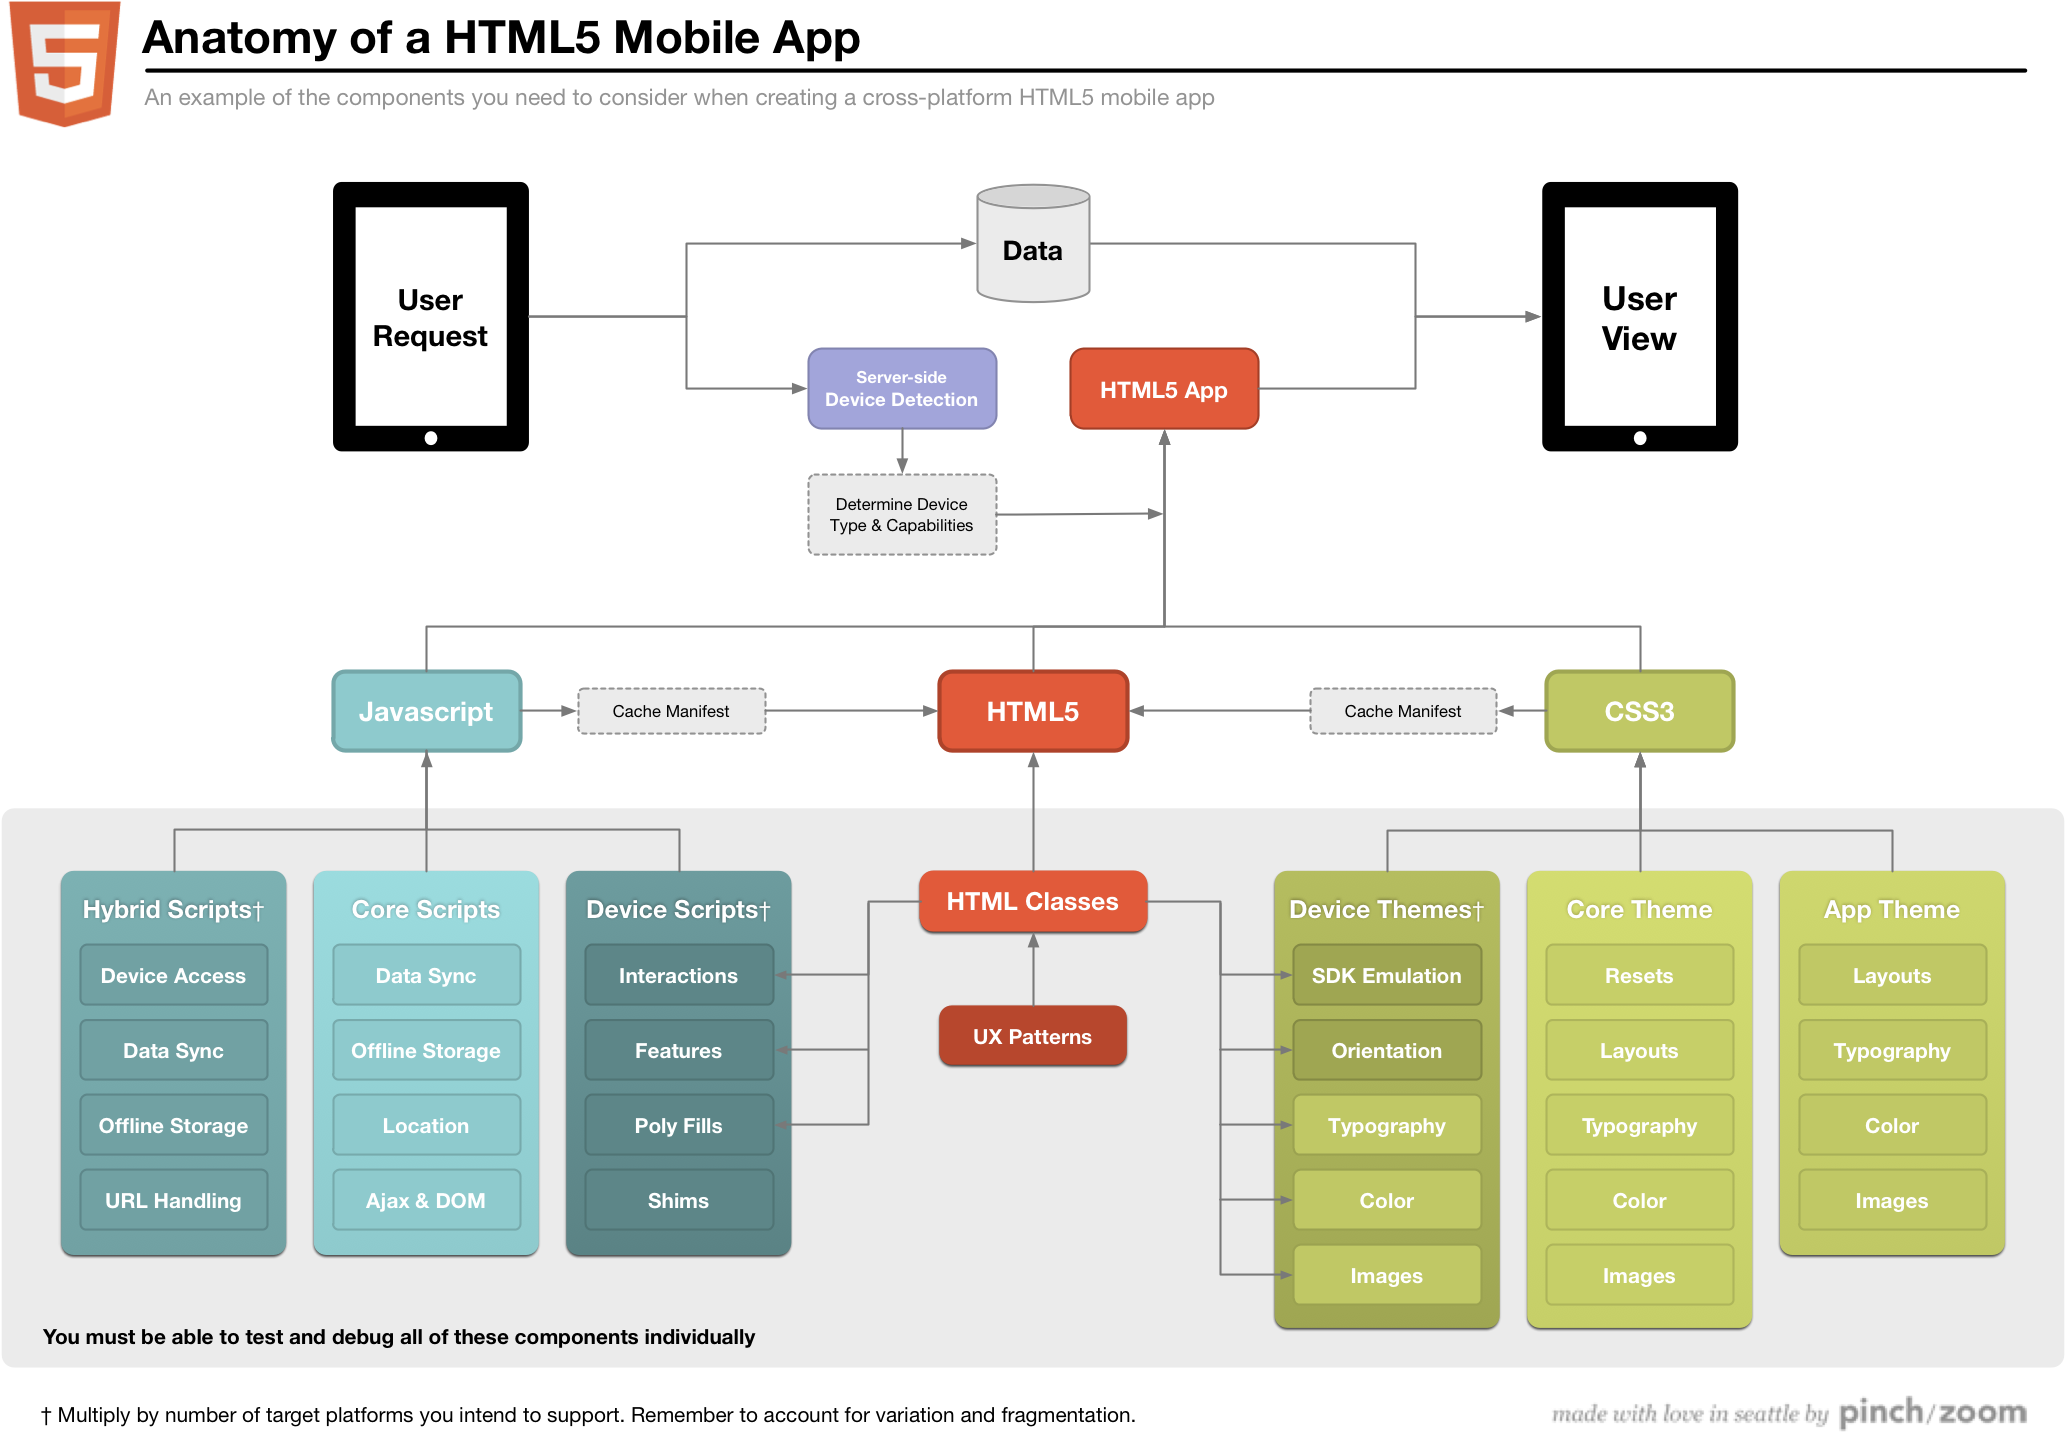
\includegraphics[width=\textwidth]{images/anatomy-of-a-html5-mobile-app.png}
  \caption{HTML5 Mobile Application Anatomy \citationneeded}
  \label{figure:anatomy-of-a-html5-mobile-app.png}
\end{figure}

\subsection{Single-Page applications}
\label{section:single-page-applications}

In recent years, the movement from traditional interlinked documents
to interactive web applications has had a profound effect on the
architecture of web applications. Traditional web sites have
structured backend architectures often with a database layer, a layer
for business logic, and a layer for generating the HTML documents from
a template. The frontend usually uses \abbr{CSS} for layout and
styling and some JavaScript for enhancing forms or some interactive
components on a page.

These conventional three-tiered web applications often use an
\abbr{MVC} \cite{gamma1995design} framework for separating the data,
logic, and presentation layers in the backend. However, the latest
trend in web application development has been having only a simple
\abbr{REST} \citationneeded API as a backend data layer, and using a
JavaScript MVC framework in the frontend. Thus the whole application
logic and presentation has moved to the client side, with the backend
only working as a data persistency layer.

Using modern JavaScript storage APIs (see
Section~\ref{section:datastorage}), even the data persistency and
application state layer can be in the client side, with backend only
working as an application and data delivery layer. In addition to the
client side data persistency, the storage APIs can be used to store
the user-specific application state.

Single-page applications might introduce bigger initial page load, but
after the startup, the network is only used when interacting with the
backend data API. This makes the applications faster and more
responsive, and minimizes the effects that unreliable networks have on
the application usage since separate page views do not require a new
document request.

\subsubsection{JavaScript MVC Libraries}
\label{section:js-mvc}

Due to the recent trend to move application logic from the backend to
the frontend, JavaScript code bases have grown into large applications
that need a proper modular structure. Several frameworks have been
developed to structure JavaScript applications into well-separated
modules and layers.

Many of the JavaScript application frameworks are derived from the MVC
architecture pattern adapting it to the design needs and requirements
of browser-based applications. Example frameworks include
Backbone.js\footnote{\url{http://backbonejs.org/}},
Spine\footnote{\url{http://spinejs.com/}},
batman.js\footnote{\url{http://batmanjs.org/}},
Knockout\footnote{\url{http://knockoutjs.com/}}, and
JavaScriptMVC\footnote{\url{http://javascriptmvc.com/}}.

One popular framework nowadays is Backbone.js, which we also chose for
the application described in
Chapter~\ref{chapter:methods}. Backbone.js is an open source
JavaScript framework providing the essential components and structures
for building large JavaScript applications. Backbone.js provides the
following components:

\begin{itemize}
\item \textbf{Model}

  Models provide the domain-specific data layer of the
  application. They provide data manipulation, persistency, and
  serialization methods as well as an event handling mechanism for
  data changes.

\item \textbf{Collection}

  Collections are ordered sets of models. They can be used to observe
  and manipulate models as a group. They can also be used to filter
  specific models for some purposes.

\item \textbf{Router}

  Routers provide methods for routing between pages of an application
  by observing and modifying the \abbr{URL}. URLs can be mapped to
  events and actions for client-side application navigation.

\item \textbf{History}

  The History utility is used together with Routers to handle the
  application navigation to preserve the back button functionality and
  the bookmarking of certain pages in the application.

\item \textbf{Sync}

  The Sync utility provides data synchronization to the backend.

\item \textbf{View}

  Views are structures that help organizing the user interface into
  logical parts. They usually observe certain models or collections
  for changes, and update themselves independently of each other when
  the underlying data changes. They are often used together with some
  templating library, such as
  Mustache\footnote{\url{http://mustache.github.com/}} or
  Handlebars\footnote{\url{http://handlebarsjs.com/}}.

\end{itemize}

\subsection{Responsive Design}

Responsive design is a way to design a web page to fit to varying
sizes of screens and devices. The traditional way to design a web page
is to compromise on a certain width based on the expected desktop
screen sizes of the target audience and to lay out the elements of the
page to the chosen width.

Using Media Queries (see Section~\ref{section:css}), we can provide
tailored layouts for different screen sizes. For example, we can swap
the images to smaller ones for mobile devices or hide some elements to
make the layout cleaner on small screens. This enables us to use the
same code base to target all devices and screens.

\subsection{Progressive Enhancement}
\label{subsection:progressive-enhancement}

Modern web sites and web applications are accessed with a huge variety
of devices and form-factors with varying capabilities, and supporting
all the possible browsers your users might have becomes a huge burden
on developers. New standards support and \abbr{APIs} in latest
browsers seem tempting and valuable, but having to support also
less-capable browsers prevent developers from using a single solution
for all browsers.

The goal of progressive enhancement is to provide universal access to
a web site or application no matter what capabilities the browser of
the user has. Parker et al. define the three key principles of
progressive enhancement \cite{parker2010designing}:

\begin{itemize}
\item Start with clear content and well-structured markup.
\item Maintain strict separation of layout and presentation.
\item Unobtrusively layer in advanced behavior and styling, with
  careful consideration of accessibility implications.
\end{itemize}

Often the design is started ``mobile first'' meaning that the simplest
and the most universal bottom layer of the application is designed for
the least-capable browsers with very little screen estate. This forces
the design to be simple and semantic, and filters out any extra markup
that is not needed for the semantic presentation of the content and
functionality. In addition, by designing first to browsers that might
not even have \abbr{CSS} support forces a clear separation of layout
and content as well as makes the clean markup easier to style and
enhance \cite{parker2010designing}.

Using feature detection (see Section~\ref{section:feature-detection}),
more layers are added on top of the clean markup. The objective is to
use unobtrusive JavaScript to enhance the markup to avoid breaking
parts of the page or the whole site with careless scripting. By using
feature detection, we ensure that we take the most out of the latest
browsers by using their full capabilities, and at the same time,
keeping the application accessible and functional in less-capable
browsers. This also makes the applications future-proof when browsers
are updated and new APIs and features are implemented in
them. \cite{parker2010designing}

\subsection{UI Libraries}

\subsubsection{jQuery Mobile}

jQuery Mobile \footnote{\url{http://jquerymobile.com/}} is a client
side framework optimized for touch devices. The user interface is
based on HTML5 and the jQuery JavaScript
framework\footnote{\url{http://jquery.com/}}. The aim of the project
is to provide a progressively enhanced web framework for as many
devices as possible. Figure~\ref{figure:jquerymobile.png} shows
example components in the framework.

\begin{figure}[ht]
  \begin{center}
    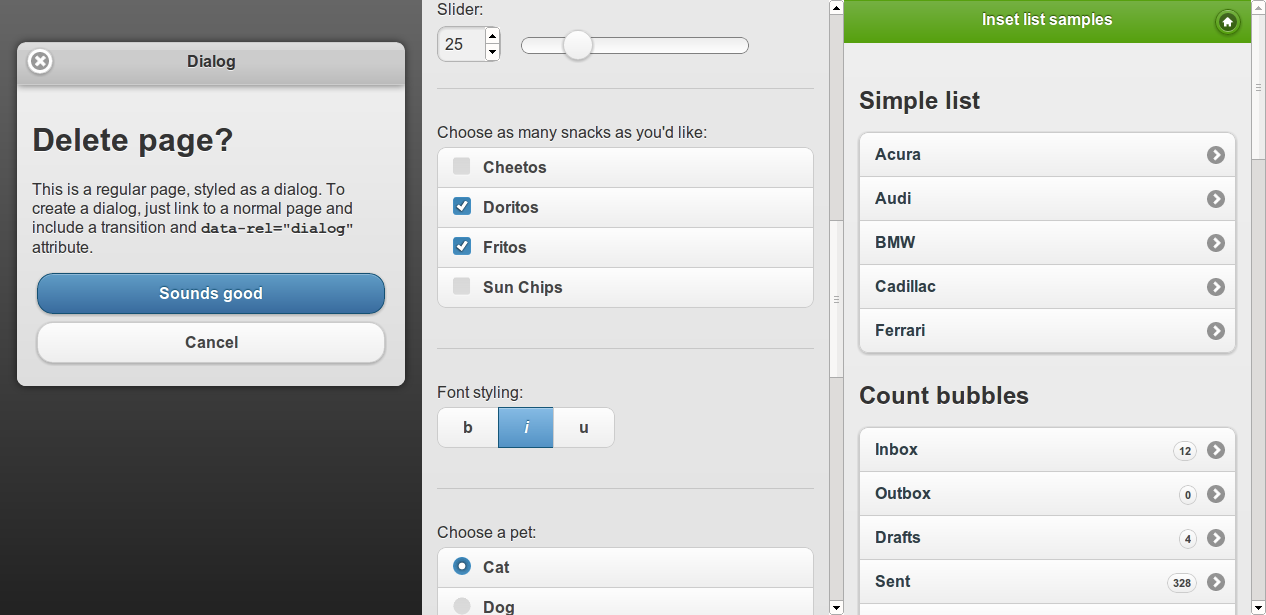
\includegraphics[width=\textwidth]{images/jquerymobile.png}
    \caption{jQuery Mobile user interface
      components. \url{http://jquerymobile.com/demos/1.0.1/}}
    \label{figure:jquerymobile.png}
  \end{center}
\end{figure}

jQuery Mobile is an open source project sponsored by large mobile and
media companies. The user interface is fully theamable and there are
several third-party extensions and widgets to the framework.

\subsubsection{jQTouch}

jQTouch \footnote{\url{http://jqtouch.com/}} is a lightweight open
source library for high-end smartphones and tablet devices. It only
supports the WebKit browser
engine \footnote{\url{http://www.webkit.org/}} used in iOS, Android,
Blackberry, and WebOS devices. It provides customizable themes and
user interface components, as well as helpers for handling touch
input. Figure~\ref{figure:jqtouch.png} shows example components of the
library.

\begin{figure}[ht]
  \begin{center}
    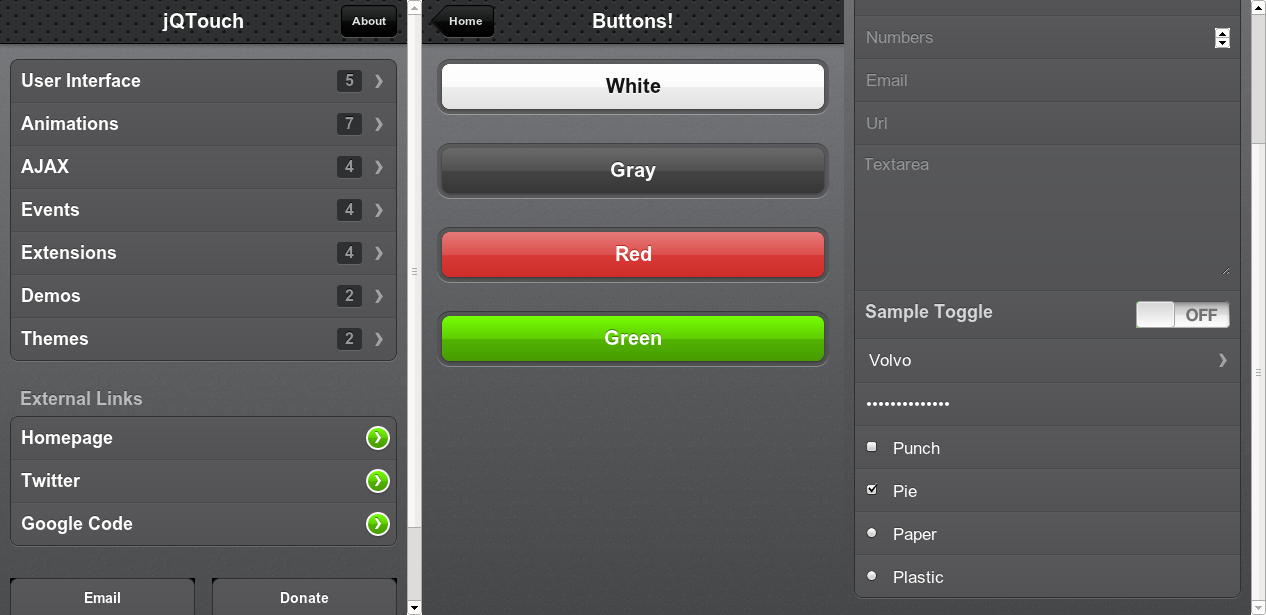
\includegraphics[width=\textwidth]{images/jqtouch.png}
    \caption{jQTouch user
      interface. \url{http://jqtouch.com/preview/demos/main/}}
    \label{figure:jqtouch.png}
  \end{center}
\end{figure}

\subsubsection{Sencha Touch}

Sencha Touch is an open source HTML5 mobile web application framework
for iPhone, Android, and Blackberry devices. The framework is fully
theamable and comes with a large set of user interface components. It
also provides helpers for touch input
handling. Figure~\ref{figure:sencha.png} shows example components of
the library.

\begin{figure}[ht]
  \begin{center}
    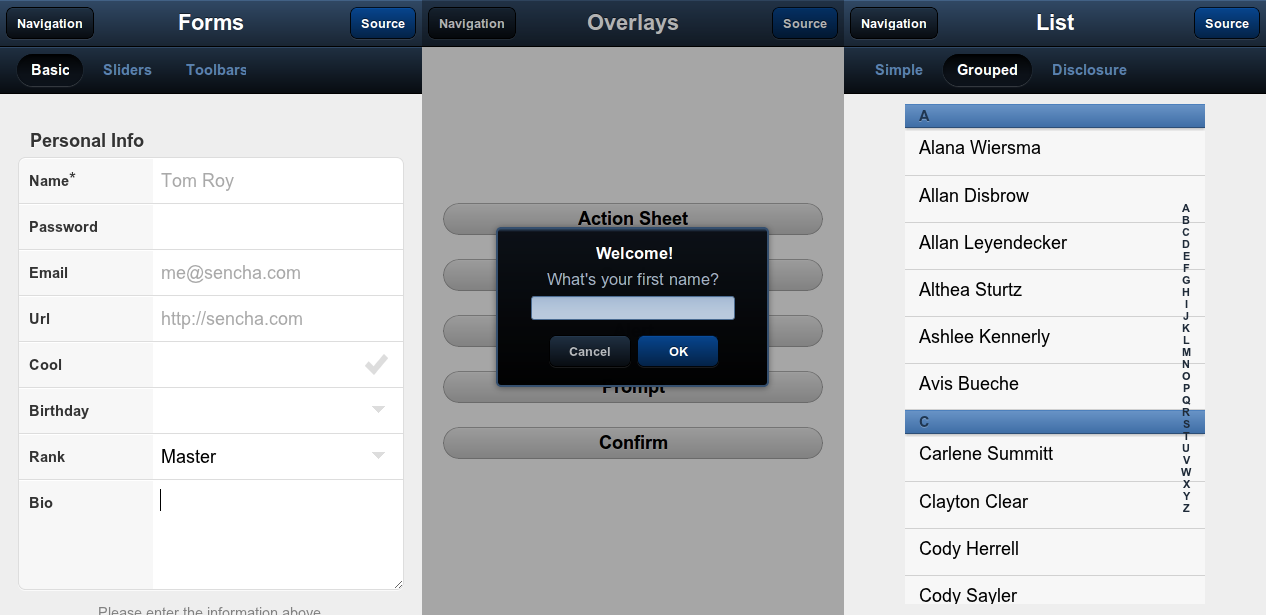
\includegraphics[width=\textwidth]{images/sencha.png}
    \caption{Sencha Touch user
      interface. \url{http://dev.sencha.com/deploy/touch/examples/kitchensink/}}
    \label{figure:sencha.png}
  \end{center}
\end{figure}

\subsection{Hybrid Applications}

Sometimes application stores can be a valuable marketing path, and
visibility in these stores can bring a lot of users to an
application. The stores also provide easy billing of applications
themselves, and solutions for in-app billing. \citationneeded

Fortunately, modern smartphone and tablet platforms provide a user
interface component to embed a web browser view into a native
application. This web view component can be used to build parts or
even the whole application with web technologies. For example, the web
view can take the whole available screen space of the application, and
show a local HTML document together with local assets like CSS and
JavaScript files and images.

These applications that use a native web view wrapper with parts of
the application built with web technologies are called hybrid
applications. The level of native versus web technologies can vary,
and everything is possible from fully utilizing web technologies with
just a simple native wrapper to a native application with just a
simple static HTML document.

Several tools have been developed to build hybrid applications. One of
these is PhoneGap \footnote{\url{http://phonegap.com/}}, which is an
open source HTML5 application platform for building native
applications with web technologies. PhoneGap provides native wrappers
for all of the largest mobile platforms, and exposes extra JavaScript
APIs that are not accessible in normal web pages. These APIs are based
on the latest specifications, and they can be used to access device
functionality that has previously been inaccessible using JavaScript.

With tools like PhoneGap, developers can build native applications
using familiar web technologies with access to native features and
device APIs. These hybrid applications have only one code base that is
deployed for several smartphone platforms, and the applications can be
submitted to application stores.

\clearpage
\section{Performance Guidelines}
\label{section:performance-guidelines}

There are several web application performance best practices and
related guidelines. According to Souders \cite{souders2007high}, only
10--20\% of the end user response time is spent generating and
transferring the HTML document from the web server to the
client. Therefore, most of the optimization should be done in the
frontend for best improvement opportunities. Below we list the
performance guidelines defined by Souders \cite{souders2007high}.

\begin{itemize}

  % High Performance Web Sites

\item \textbf{Make Fewer HTTP Requests}

  According to Souders, 80--90\% of the end user response time is
  spent downloading components in a page other than the requested HTML
  page. Therefore, the simplest way to improve the response time is to
  reduce the number of HTTP requests needed to get all the required
  components.

  There are several ways to reduce the number of needed HTTP
  requests. Combining images into sprites, inlining images, or
  combining separate JavaScript and CSS files results in fewer
  components needed to download on a page.

\item \textbf{Use a Content Delivery Network}

  As web applications are deployed and become accessible worldwide,
  latency might become an issue for users far from the application's
  web servers. Geographically distributed servers allow for serving
  the application as close to the user as possible.

\item \textbf{Add an Expires Header}

  Avoiding a HTTP request altogether is the best option for reducing
  the response time when downloading the components in a page. Good
  caching strategies help browsers to know which resources are valid
  and for how long until they should be updated.

  The Expires header in HTTP tells the client how long a resource is
  valid, and especially far future Expires headers reduce the need for
  downloading and updating the components in a page after the initial
  download.

\item \textbf{Gzip Components}

  Compressing HTTP responses is an easy and effective way to reduce
  the size of the data needed to transfer across the
  network. Compression is supported widely in web browsers and the
  impact of reduced response sizes is huge. Using Gzip, the response
  size is reduced generally about 70\%.

\item \textbf{Put Stylesheets at the Top}

  Putting the CSS files to the top of the document allows the page to
  load progressively and the browser to show visual feedback to the
  user as early as possible.

\item \textbf{Put Scripts at the Bottom}

  Because scripts block parallel downloads, they should be included to
  the page after all other resources. They also block progressive
  rendering of all content below them in the HTML document, and should
  therefore be at the bottom of the document.

\item \textbf{Avoid CSS Expressions}

  CSS expressions are a way to dynamically set CSS properties in
  Internet Explorer by evaluating a JavaScript code in a
  stylesheet. However, despite the obvious upsides, the expressions
  are evaluated at such a high frequency that they negatively impact
  the performance.

\item \textbf{Make JavaScript and CSS External}

  There are performance tradeoffs between making JavaScript and CSS
  external versus inlining them in the HTML document. In the typical
  case, however, making them external enables the browser to leverage
  the HTTP caching semantics and thus reduces the needed network
  transfer.

\item \textbf{Reduce DNS Lookups}

  Apart from cached \abbr{DNS} lookups, the browser typically needs
  20--120 milliseconds to look up the \abbr{IP} address for a given
  hostname. The cache lifetime of a lookup depends on the \abbr{TTL}
  value of the DNS record and having the components of a page
  distributed across several domains might accumulate into a
  noticeable response time.

  There is also a trade-off between unique hostnames and allowed
  parallel connections and therefore these settings should be
  configured based on the application architecture and needs.

\item \textbf{Minify JavaScript}

  Because JavaScript is an interpreted language that must be sent to
  the web browser as source code, minifying the code reduces the
  required network transfer. Minifiers and obfuscators optimize the
  size of the source code by stripping extra whitespace and comments
  as well as renaming variables and function names to shorter ones
  without changing the interpreted behavior of the code.

\item \textbf{Avoid Redirects}

  Rerouting any component in a page takes time, and avoiding any kind
  of redirects improves the response times.

\item \textbf{Remove Duplicate Scripts}

  Including a resource several times serves no purpose but is actually
  quite common. Developers should make sure to include resources only
  once.

\item \textbf{Configure ETags}

  \abbr{ETags} are a mechanism in HTTP for servers and browsers to
  validate cached resources. The typical default values set by
  commonly used web servers might hurt performance, and should thus be
  configured properly to address the application architecture and
  needs.

\item \textbf{Make Ajax Cacheable}

  Highly dynamic web sites have a lot of \abbr{Ajax}
  \cite{garrett2005ajax} functionality, and developers should make
  sure all the requested URLs for data fetching follow the performance
  best practices such as having proper caching in place.

\end{itemize}

In addition to the performance rules \cite{souders2007high}, Souders
also specifies additional techniques to improve performance
\cite{souders2009even}:

\begin{itemize}

  % Even Faster Web Sites

\item \textbf{Splitting the Initial Payload}

  Nowadays, web sites include a lot of resources and JavaScript
  functionality, but only a small part of the downloaded components
  are used in the typical use cases of the application. Splitting the
  resources into bundles that can be lazily downloaded when first
  needed reduces the initial payload needed to transfer on application
  startup.

\item \textbf{Loading Scripts Without Blocking}

  Most browsers block the downloads of other resources when scripts
  are being downloaded and executed. There are several ways to
  circumvent this behavior to allow browsers download scripts in
  parallel with other resources as well as with other script files.

\item \textbf{Coupling Asynchronous Scripts}

  Related to the previous item, when using parallel downloads with
  scripts that are dependent on each other, race conditions might
  occur due to the varying order of download and execution. Therefore,
  asynchronous scripts dependent on each other should be coupled to
  preserve the correct order of execution.

\item \textbf{Positioning Inline Scripts}

  Inline scripts do not introduce an HTTP request, but they can still
  block parallel downloads of other resources and they might affect
  also the progressive rendering of the page. With the correct
  positioning of the scripts, these problems can be handled properly.

\item \textbf{Writing Efficient JavaScript}

  After networking, the obvious place to optimize the runtime speed of
  a web application is the JavaScript code.

  Because the whole user interface and the JavaScript code run in the
  same browser thread, there can be only one thing happening at a
  time. Long running functions block the user interface from updating
  and can result in bad user experience.

  Splitting the running code into properly sized chunks, appropriately
  leveraging the asynchronous patterns of JavaScript in the
  application architecture, understanding the details and slow parts
  of the DOM API, and using several JavaScript programming best
  practices can result in big improvements in the perceived
  application performance. \cite{zakas2010high}

\item \textbf{Scaling with Comet}

  For real-time data-driven applications, there are various
  optimization techniques related to optimizing the constant data
  transfer between the server and the client. The collection of there
  various technologies is unofficially called Comet.

\item \textbf{Going Beyond Gzipping}

  Although Gzipping is widely supported in web browsers, there are
  cases when it is not supported or when the support is not
  indicated. Stripping extra content such as unneeded whitespace and
  comments reduces the payload size for uncompressed responses. There
  are also ways to detect Gzip support if the client does not directly
  indicate that.

\item \textbf{Optimizing Images}

  Images typically tend to account for a large portion of the page
  weight, and since the page weight is highly correlated to the
  response time, images are a natural target for optimization. There
  are several ways to optimize images either with lossy or lossless
  conversions.

\item \textbf{Sharding Dominant Domains}

  By tuning the amount of unique hostnames used for serving all the
  resources of an application, parallel downloads can be better
  leveraged. Also, by using HTTP 1.0 with proper Keep-Alive headers or
  HTTP 1.1 with proper persistent connections the parallel downloads
  can be tuned for better performance.

\item \textbf{Flushing the Document Early}

  Some web application frameworks allow flushing parts of the document
  to the user before the whole document is generated. This enables
  progressive rendering and gives faster feedback to the user and thus
  improves the perceived performance.

\item \textbf{Using Iframes Sparingly}

  Iframes enable developers to embed a separate HTML document inside
  another document. They are useful in sandboxing external documents
  in the same view, but the \texttt{iframe} element is the most
  expensive DOM element related to the page performance.

\item \textbf{Simplifying CSS Selectors}

  There are several ways to choose elements in CSS stylesheets to
  apply the defined properties to. Some selectors are faster than
  others and some have terrible performance.

\end{itemize}
